\documentclass[a4paper, 11pt]{article}
\usepackage{comment} % enables the use of multi-line comments (\ifx \fi) 
\usepackage{fullpage} % changes the margin
\usepackage{pdflscape}
\usepackage{rotating}
\usepackage{graphicx}
\usepackage[table]{xcolor}

\begin{document}
%Header-Make sure you update this information!!!!
\noindent
\large\textbf{Program Assignment 2} \hfill \textbf{Longxiang Li} \\
\normalsize CS124 \hfill Teammates: Fangyuan Hong \\

\section*{Introduction}
Strassen's matrix multiplication algorithms works faster for $n$ by $n$ matrix than the conventional naive algorithm whose time complexity is $O(n^3)$, in theory. However, for some smaller n, the conventional algorithm runs faster because the time consumed in memory allocation in Strassen's algorithm. But, for this recursive algorithm, we don't need to go to the basic element of this matrix (a $1\times1$). We may modified the classic algorithm by converting from recursion to conventional algorithm when the dimension is small enough. We call this cross-over point. In this experiment, we try to find the optimal cross-over point for different $n$ from two direction. First, we calculate the exact running time for Strassen's algorithm, modified Strassen's algorithm and conventional algorithm and estimate the cross-over point numerically. These calculation were based on the assumption that the cost of any single arithmetic operation is 1 and all others are free. Second, we implemented these algorithms and get the cross-over point in practice.
\section*{Numerical Analysis of cross-over point}
To simplify the calculation we assume in the following analysis in this section, the dimension n is power of 2 and the cross-over value is also power of 2. In classic Strassen's algorithm, for a given matrix of given $n$, we require 7 multiplication of matrices of simension $\frac{n}{2}$. In addition, there are 18 summation and subtraction of size $\frac{n}{2}$. Thus, we can write a recursive equation of the running time:
\[{f_1}(n)=7f(\frac{n}{2})+18(\frac{n}{2})^2\] 
\[=7^2f(\frac{n}{4})+7\times18 (\frac{n}{4})^2+18(\frac{n}{2})^2\] 
\[=7^kf(\frac{n}{2^k})+18n^2\{7^{k-1}(\frac{1}{2^k})^2+\dots+7^0(\frac{1}{2})^2\}\]
when $k=log_2{n}$, we arrive at the basic case. Since $f(1)=1$. We can conclude that the exact running time of standard Strassen's algorithm is:
\[f_s(n)=7^{log_2{n}}+6n^2\{(\frac{7}{4})^{log_2{n}}-1\}\]
For conventional algorithm, we have a total of $n^3$ multiplication and $n^2(n-1)$ additions. So the close form running time of conventional algorithm is:
\[f_c(n)=n^2(2n-1)\]
Let's assume we set cross-over point at $n_0$. That means above $n_0$, we used Strassen's algorithm and below $n_0$, we used conventional algorithm. So the running time of this hybrid algorithm is:
\[f_{n_0}=7^{log_2{\frac{n}{n_0}}}(2n_0^3-n_0^2)+6n^2((\frac{7}{4})^{log_2{\frac{n}{n_0}}}-1)\]
\begin{figure}
	\centering
	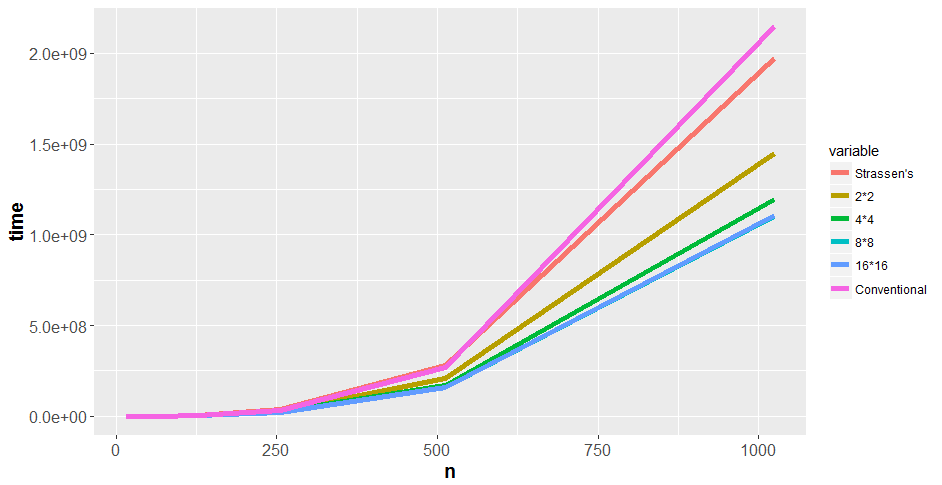
\includegraphics[width=0.9\linewidth]{TRuntimemulti}
	\caption{Theoretical runtime of standard Strassen's, conventional algorithm and modified Strassen's with cross-over value ranging from 2 to 16 }
	\label{fig:truntimemulti}
\end{figure}

We cannot achieve a closed form $n_0$ for every $n$. But we can get a numeric estimation. The theoretical running time of standard Strassen's, modified Strassen's with $2\times2$, $4\times4$, $8 \times 8$, $16 \times 16$ basic matrix and conventional algorithm are listed below:
\begin{table}[ht]
	\centering
	\caption{Theoretical runtime of standard Strassen's, conventional algorithm and modified Strassen's with cross-over value ranging from 2 to 16}
	\begin{tabular}{rrrrrrrr}
		\hline
		& n & Strassen's & 2*2 & 4*4 & 8*8 & 16*16 & Conventional \\ 
		\hline
		 & 16 & 15271 & 10812 & 8656 &\cellcolor{blue!25} 7872 & 7936 & 7936 \\ 
	 & 32 & 111505 & 80292 & 65200 &\cellcolor{blue!25}  59712 & 60160 & 64512 \\ 
		& 64 & 798967 & 580476 & 474832 &\cellcolor{blue!25}  436416 & 439552 & 520192 \\ 
		 & 128 & 5666497 & 4137060 & 3397552 &\cellcolor{blue!25}  3128640 & 3150592 & 4177920 \\ 
		 & 256 & 39960391 & 29254332 & 24077776 &\cellcolor{blue!25}  22195392 & 22349056 & 33488896 \\ 
		 & 512 & 280902385 & 205959972 & 169724080 &\cellcolor{blue!25}  156547392 & 157623040 & 268173312 \\ 
		 & 1024 & 1971035287 & 1446438396 & 1192787152 &\cellcolor{blue!25}  1100550336 & 1108079872 & 2146435072 \\ 
		\hline
	\end{tabular}
\end{table}
For a matrix with size of $n$, when $n\leq 16$, by no means can Strassen's run faster than conventional algorithm in theory. However, if we chose a cross-over point at 8, the modified Strassen's algorithm consume fewer calculation operation than the conventional algorithm. This is true for other matrix dimension. Because if the dimension of a matrix is a power of 2, the cross-over points should also be powers of 2. So, at least when $n<2^{12}$, $n_0=8$ according to numeric analysis.
In this plot, we could find the cross-over point is located at $8\times8$ for both matrix size of 4096 and matrix size of 256.
\begin{figure*}[h]
	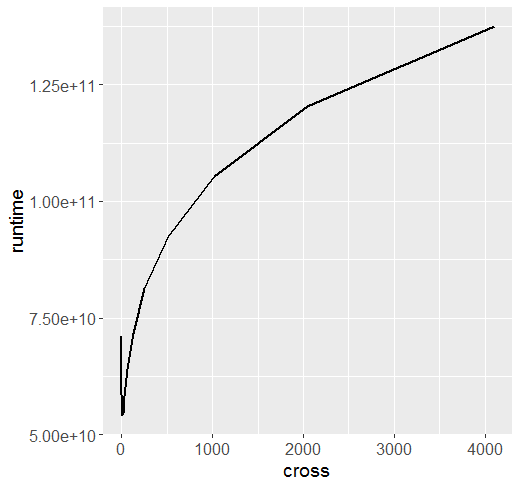
\includegraphics[width=0.5\linewidth]{Truntime}
	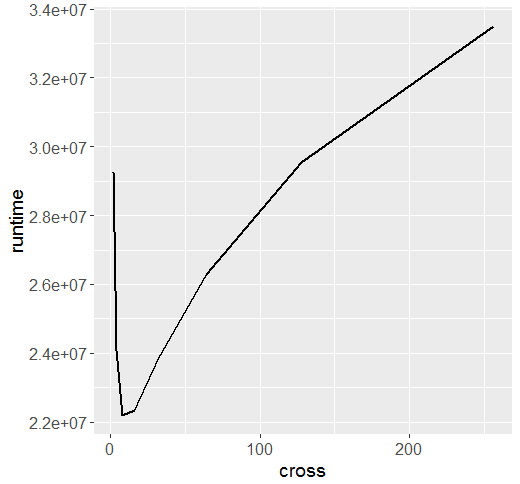
\includegraphics[width=0.5\linewidth]{Truntime8}
	\caption{Theoretical runtime of matrix multiplication by modified Strassen's algorithm of different cross-over points}
	\label{fig:truntime}
\end{figure*}

\section*{Implementation}
Our implementation was straightforward, similar with what is given in class.

 First, We created utility functions matrix sum, matrix subtract, matrix initiation and matrix release. Then we implement the conventional algorithm. According to the hint, there's a performance difference between column first implementation and row first implementation. We found that column first implementation ran faster. So this implementation was applied here. Subsequently, we implemented the Strassen's algorithm. To begin with, we created a function to divide our matrix into four sub-matrix equally. After splitting, we utilized the functions created above to implement the addition and multiplication. Finally, the four sub-matrix were merged as output. After doing these calculation, all memories were released.

However, this implementation only works when dimension is power of 2, indicating the dimension can be divided by 2 recursively. In other dimensions, when the dimension is odd, we tab one row of zeros at the bottom and one column of zero at right end to make the dimension dividable by 2 again. This is very different from tabbing zeros to the next power of 2 dimension. After running a standard Strassen's on this extended matrix, we extracted the left-upper $n*n$ elements as output.We tested this algorithm in experiment and proved this is correct by comparing with conventional algorithm's result. 

\section*{Experimental analysis of cross-over point}
We took record of the running time of our implementation on matrices of size of 1024, 1025, 2048, 2049 with cross-over values ranging from 8 to 296 at interval 8 for first two smaller matrix and with cross-over values ranging from 8 to 392 at interval 8 . We ran 5 trails for each cross-over value for each matrix and took the average. All times are given in seconds here. Full record were shown in attachment.
\begin{figure*}[ht]
	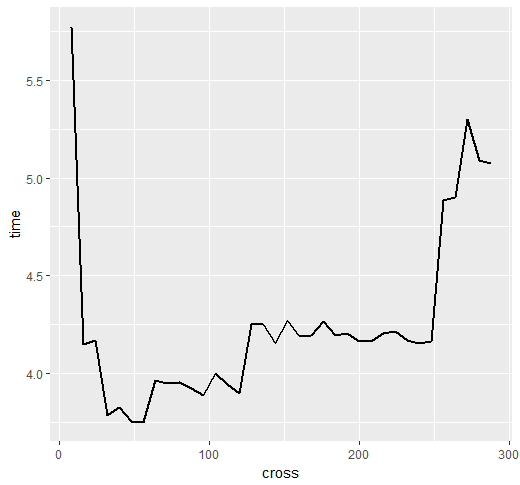
\includegraphics[width=0.5\linewidth]{Actual1024}
	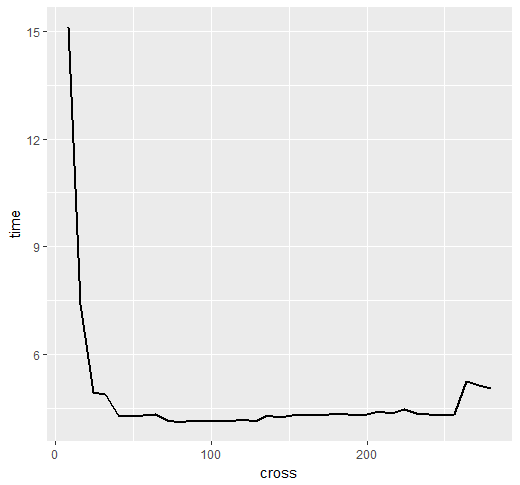
\includegraphics[width=0.5\linewidth]{Actual1025}
	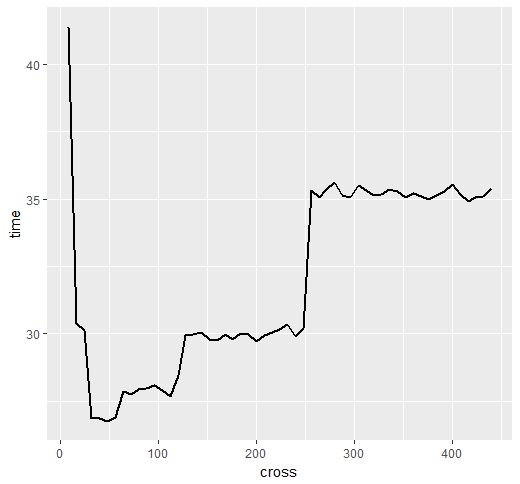
\includegraphics[width=0.5\linewidth]{Actual2048}
	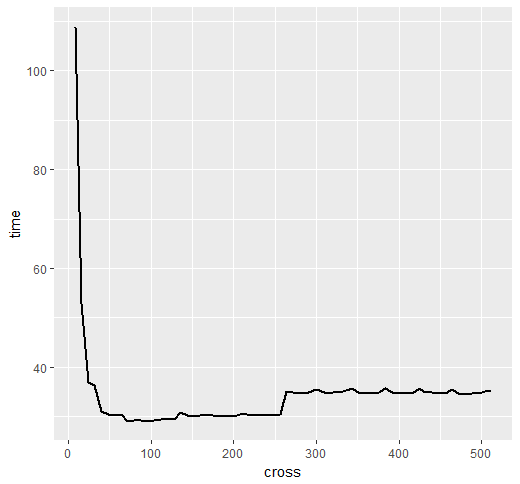
\includegraphics[width=0.5\linewidth]{Actual2049}
	\caption{Exprimental run time of modified Strassen's on matrix size of 1024(upper left), 1025 (upper right), 2048 (lower left), 2049 (lower right)}
	\label{fig:truntime}
\end{figure*}
We can extract the lowest point for each plot and treat it as experimental cross-over point.
\begin{table}[h]
	\centering
	\caption{Exprimental cross-over value for matrix size 1024, 1025, 2048, 2049}
	\begin{tabular}{|c|c|c|c|c|}
		\hline 
		Matrix Dimension& Experimental Cross-over&RT of modified Stra& RT of Stra&RT of conven \\ 
		\hline 
		1024& 48-56& 3.75&113.274&\\ 
		\hline 
		1025& 88-96& 4.12&754.387&\\ 
		\hline 
		2048& 48-56& 26.75&1306.62&\\ 
		\hline 
		2049& 88-96& 29.13&&\\ 
		\hline 
	\end{tabular} 
\end{table}
From these plots and table, we can find that the running time decrease quickly af first when small basic matrix was introduced in the modified Strassen's algorithm. But as the size of basic basic matrix increase, the running time goes up. Here the increasing trend for matrix size of power of 2 and not power of 2 are very different. For matrix size of power of 2, the running time varies at every crossover value of power of 2. But due to the limited trail number, there are some variations at values not power of 2. We can also see here the performance difference of different tabbing method. In the worst cases such as a matrix size of 1025 (power of 2 and another 1), if we tabbed zero to the next power of 2, the running time will be close to the running time of matrix of 2048. Almost 8 times the running time of matrix size of 1024. But with our implementation, even though slower than the matrix of 1024 due to more memory allocation and calculation, they're similar. At the same time, we can also compare the experimental runtime of standard Strassen's algorithm and conventional algorithm.

\section*{Discussion}
In the above parts, we tried to estimate the optimal cross-over value in two ways: analytically and experimentally. The result of numerical analysis is 8 while the result of experimental analysis is different, for matrix size of power of 2, the crossover value ranges from 48 to 56 while for matrix size not power of 2, the crossover value ranges from 88 to 96. We need to discuss this discrepancy. First, we assume only arithmetic operation cost time and all other operations are free. This is surreal because allocating memory and releasing memory cannot be free. As a result, this may encourage us to convert to conventional algorithm earlier than analytical result. Second, not all arithmetic operation are identical in fact. But the influence of this inequity is unclear.

 
\section*{Appendix}
\begin{table}[ht]
	\centering
	\begin{tabular}{rrrr}
		\hline
		index& $n_0$ & n=2048 & n=2049 \\ 
		\hline
		1 & 8 & 41.40 & 108.83 \\ 
		2 & 16 & 30.37 & 52.89 \\ 
		3 & 24 & 30.13 & 36.84 \\ 
		4 & 32 & 26.85 & 36.27 \\ 
		5 & 40 & 26.86 & 31.17 \\ 
		6 & 48 & 26.75 & 30.39 \\ 
		7 & 56 & 26.87 & 30.31 \\ 
		8 & 64 & 27.85 & 30.42 \\ 
		9 & 72 & 27.73 & 29.15 \\ 
		10 & 80 & 27.95 & 29.26 \\ 
		11 & 88 & 27.96 & 29.25 \\ 
		12 & 96 & 28.09 & 29.13 \\ 
		13 & 104 & 27.89 & 29.26 \\ 
		14 & 112 & 27.69 & 29.45 \\ 
		15 & 120 & 28.43 & 29.59 \\ 
		16 & 128 & 29.93 & 29.55 \\ 
		17 & 136 & 29.98 & 30.77 \\ 
		18 & 144 & 30.05 & 30.35 \\ 
		19 & 152 & 29.80 & 30.13 \\ 
		20 & 160 & 29.77 & 30.21 \\ 
		21 & 168 & 29.98 & 30.47 \\ 
		22 & 176 & 29.77 & 30.21 \\ 
		23 & 184 & 30 & 30.03 \\ 
		24 & 192 & 29.97 & 30.18 \\ 
		25 & 200 & 29.71 & 30.07 \\ 
		26 & 208 & 29.95 & 30.56 \\ 
		27 & 216 & 30.03 & 30.52 \\ 
		28 & 224 & 30.17 & 30.25 \\ 
		29 & 232 & 30.34 & 30.29 \\ 
		30 & 240 & 29.89 & 30.37 \\ 
		31 & 248 & 30.18 & 30.34 \\ 
		32 & 256 & 35.33 & 30.38 \\ 
		33 & 264 & 35.06 & 35.17 \\ 
		34 & 272 & 35.35 & 34.92 \\ 
		35 & 280 & 35.61 & 34.79 \\ 
		36 & 288 & 35.13 & 34.79 \\ 
		37 & 296 & 35.07 & 35.29 \\ 
		38 & 304 & 35.52 & 35.34 \\ 
		39 & 312 & 35.33 & 34.75 \\ 
		40 & 320 & 35.13 & 34.83 \\ 
		41 & 328 & 35.19 & 34.92 \\ 
		42 & 336 & 35.37 & 35.36 \\ 
		43 & 344 & 35.27 & 35.63 \\ 
		44 & 352 & 35.08 & 34.81 \\ 
		45 & 360 & 35.23 & 34.73 \\ 
		46 & 368 & 35.09 & 34.80 \\ 
		47 & 376 & 34.99 & 34.91 \\ 
		48 & 384 & 35.15 & 35.66 \\ 
		49 & 392 & 35.28 & 34.83 \\ 
		\hline
	\end{tabular}
\end{table}

\begin{table}[ht]
	\centering
	\begin{tabular}{rrrr}
		\hline
		& $n_0$ & n=1024 & n=1025 \\ 
		\hline
		1 & 8 & 5.77 & 15.12 \\ 
		2 & 16 & 4.15 & 7.39 \\ 
		3 & 24 & 4.17 & 4.93 \\ 
		4 & 32 & 3.78 & 4.88 \\ 
		5 & 40 & 3.82 & 4.31 \\ 
		6 & 48 & 3.75 & 4.26 \\ 
		7 & 56 & 3.75 & 4.29 \\ 
		8 & 64 & 3.96 & 4.33 \\ 
		9 & 72 & 3.95 & 4.15 \\ 
		10 & 80 & 3.95 & 4.12 \\ 
		11 & 88 & 3.92 & 4.15 \\ 
		12 & 96 & 3.89 & 4.14 \\ 
		13 & 104 & 4 & 4.16 \\ 
		14 & 112 & 3.94 & 4.13 \\ 
		15 & 120 & 3.90 & 4.18 \\ 
		16 & 128 & 4.25 & 4.13 \\ 
		17 & 136 & 4.25 & 4.29 \\ 
		18 & 144 & 4.15 & 4.26 \\ 
		19 & 152 & 4.27 & 4.31 \\ 
		20 & 160 & 4.19 & 4.33 \\ 
		21 & 168 & 4.19 & 4.31 \\ 
		22 & 176 & 4.26 & 4.32 \\ 
		23 & 184 & 4.20 & 4.35 \\ 
		24 & 192 & 4.20 & 4.29 \\ 
		25 & 200 & 4.16 & 4.34 \\ 
		26 & 208 & 4.16 & 4.40 \\ 
		27 & 216 & 4.20 & 4.36 \\ 
		28 & 224 & 4.21 & 4.46 \\ 
		29 & 232 & 4.17 & 4.35 \\ 
		30 & 240 & 4.15 & 4.31 \\ 
		31 & 248 & 4.16 & 4.29 \\ 
		32 & 256 & 4.88 & 4.34 \\ 
		33 & 264 & 4.90 & 5.25 \\ 
		34 & 272 & 5.30 & 5.14 \\ 
		35 & 280 & 5.09 & 5.06 \\ 
		\hline
	\end{tabular}
\end{table}
\end{document}
